\chapter{System architecture and certificate lifecycle}
\label{Architecture}

This chapter presents the architectural design decisions and  operational flows 
of the Certificate Authority. The focus is on explaining how the various 
components interact throughout the complete certificate lifecycle, from initial 
identity commitment to certificate issuance, renewal, and revocation.


\section{Source code structure}

The system consists of four primary components, each serving a specific role in 
the certificate lifecycle:

\subsection{CA backend server} 
The core service responsible for all cryptographic operations and certificate 
lifecycle management. Go was selected for its strong and complete cryptographic standard library, 
excellent performance characteristics and simplicity of development.

\subsection{User interface}
A React-based frontend providing certificate management capabilities. As this UI is intended 
to be used only for demo purposes, Next.js was chosen for its ease of use, built-in routing 
and vast ecosystem of libraries.

\subsection{Database}
Persistent storage for certificates and revocation lists. We decided to use MongoDB for its
document-oriented structure, which allows flexible storage and suits well with the certificate and 
metadata requirements. It also provides indexing capabilities for efficient 
querying and retrieval of certificate data.

\subsection{Hardware Security Module (HSM)}
We decided to use an HSM, in particular an emulated version of AWS KMS, to ensure that all CA 
cryptographic operations requiring its private key occur within FIPS 140-2 Level 3 certified hardware. 
This design decision eliminates the risk of private key exposure while providing 
enterprise-grade security and audit capabilities.

\section{Security-first architecture}
The architecture implements security principles through multiple 
layers of protection.

\subsection{Cryptographic isolation}
The CA's root private key never exists outside 
the HSM boundary. All signing operations are performed through secure API calls 
to the HSM, ensuring the key material remains protected even if other system 
components are compromised.

\subsection{Identity verification}
A two-step identity verification process combines 
email ownership verification with cryptographic proof of private key possession. 
This dual verification ensures only legitimate key owners can obtain certificates.

\subsection{Signed responses}
Critical CA responses are cryptographically signed to ensure 
integrity and authenticity. This prevents response tampering and provides 
non-repudiation for all CA operations.

\subsection{Replay protection}
Nonce-based replay protection mechanisms prevent 
malicious reuse of previously captured requests, protecting against replay attacks.

\section{Certificate lifecycle operations}

This section details the complete certificate lifecycle, explaining the message 
flows, cryptographic operations, and component interactions for each phase.

\subsection{Phase 1: identity commitment}

The certificate issuance process begins with an identity commitment phase that 
establishes and verifies user identity through a multi-step protocol.

\subsubsection{Client-side operations}

The user commits their identity by sending their public key, PEM-encoded,
along with their email address.

\subsubsection{CA backend processing}

When the CA backend receives the commitment request at the `/v1/identity` 
endpoint, it performs comprehensive validation.
The system validates the email address format using standard RFC 5322 compliance 
checking. The public key undergoes cryptographic validation 
to ensure it is valid and properly formatted.

Upon successful validation, the CA generates a unique challenge string and creates 
an identity commitment record in the database. This record contains the user's 
email, public key in DER format, challenge string and an 
expiration timestamp. The CA reserves a unique serial number for the eventual 
certificate, ensuring no conflicts occur during concurrent requests. An identity
commitment is valid for the next 24 hours, after which it expires and must be 
re-committed. In addition, it's not possible to verify the same identity twice.

\subsubsection{Email verification}

The identity verification process leverages email ownership as proof of identity. 
The CA's email service sends the challenge string, encoded in base 64, to the user's provided email 
address using a secure email delivery service.
This email-based verification serves dual purposes: it confirms the user has 
access to the claimed email address and provides the challenge string needed 
for the subsequent cryptographic proof phase.

\subsection{Phase 2: certificate generation}

The certificate generation phase requires cryptographic proof of private key 
ownership before the CA will issue a certificate.

\subsubsection{Challenge response}

After receiving the challenge via email, the user returns to the certificate 
interface and provides the challenge string. The client application retrieves 
the challenge and prompts the user to sign it using their private key.
The signing operation occurs entirely within the browser using the Web Crypto API. 
The client signs the raw challenge bytes using the private key corresponding to 
the public key submitted during commitment. This creates a digital signature 
that proves the user possesses the private key without exposing it.

\subsubsection{CA verification and certificate issuance}

The CA receives the challenge response containing the challenge string and the 
cryptographic signature. The system performs several critical verification steps.
First, the CA retrieves the identity commitment record using the provided challenge. 
It verifies the commitment hasn't expired and hasn't been previously used, 
preventing replay attacks and ensuring temporal validity.
Next, the CA performs signature verification using the public key from the 
commitment record. This cryptographic verification proves the requester possesses 
the corresponding private key. The verification process uses the appropriate 
algorithm (ECDSA or RSA) based on the committed key type.

Upon successful verification, the CA initiates certificate generation. The system 
constructs an X.509 certificate containing the user's public key, email address 
as the subject, and the reserved serial number. The certificate includes standard 
extensions such as key usage, basic constraints, and subject alternative names.

\subsubsection{HSM-Based certificate signing}

The certificate signing operation represents the most security-critical component 
of the entire system. The CA never signs certificates using local private keys; 
instead, all signing operations occur within the Hardware Security Module.
The CA formats the certificate structure and sends it to the HSM through the 
AWS KMS API. The HSM performs the cryptographic signing operation using the 
CA's root private key, which never leaves the secure hardware boundary. This 
approach ensures the highest level of security for the CA's signing operations.
The HSM returns the signature, which the CA combines with the certificate data 
to produce the final signed X.509 certificate. The completed certificate is 
returned to the client in PEM format, ready for immediate use.

\subsection{Phase 3: certificate revocation}

Certificate revocation enables certificate owners to invalidate their certificates 
before their natural expiration, essential for handling key compromise or 
changing security requirements.

\subsubsection{Revocation request authentication}

The revocation process begins when a certificate owner accesses the revocation 
interface and provides their certificate's serial number. The system requires 
cryptographic proof that the requester owns the certificate's corresponding 
private key.
The client constructs a revocation message in the format "Revoke: $<$serial number$>$" 
where the serial number matches the certificate being revoked. The user signs 
this message using their private key, creating a revocation signature that 
proves their authority to revoke the certificate. A nonce is not required in this
case because the operation can be performed only once per certificate.

\subsubsection{CA revocation processing}

The CA receives the revocation request containing the serial number and signature. 
The system retrieves the original identity commitment record associated with 
the serial number to obtain the corresponding public key.
The CA verifies the revocation signature against the constructed message 
"Revoke: $<$serial number$>$" using the certificate's public key. This verification 
ensures only the legitimate certificate owner can initiate revocation.

Upon successful verification, the CA updates the certificate record in the database, 
marking it as revoked with the current timestamp. The revoked certificate is 
immediately added to the Certificate Revocation List (CRL), making the revocation 
status publicly available through the CRL endpoint.

\subsection{Phase 4: certificate renewal}

Certificate renewal allows users to extend their certificate validity period 
without generating new key pairs, maintaining continuity while refreshing 
the certificate's temporal validity.

\subsubsection{Renewal request process}
The renewal process requires the certificate owner to prove continued possession 
of the private key. The client constructs a renewal message in the format 
"Renew: $<$serial number$>$ Nonce: $<$random nonce$>$" and signs it using the certificate's 
private key.
This signature proves the requester still controls the private key associated 
with the certificate, ensuring only legitimate certificate owners can renew 
their certificates. To avoid replay attacks, the renewal message includes a 
random nonce that must be unique for each renewal request. Subsequent requests 
for the same certificate using the same nonce will be rejected by the CA.

\subsubsection{CA renewal validation and processing}

The CA performs several validation steps before processing renewal requests.
First, the system verifies the certificate exists and hasn't been revoked. It confirms 
the certificate hasn't expired, as expired certificates cannot be renewed. 
The, the CA validates the renewal signature against the message "Renew: $<$serial number$>$ Nonce: 
$<$provided nonce$>$" using the committed public key.
Upon successful validation, the CA extends the certificate's validity period 
(typically by one year) and generates a new certificate with the updated expiration 
date. It also keeps track of the used nonces for this certificate to prevent 
replay attacks.
The renewed certificate maintains the same serial number and subject 
information while reflecting the extended validity period.

\subsubsection{HSM integration in renewal}

Similar to initial certificate issuance, the renewal process involves HSM-based 
signing operations. The CA constructs the renewed certificate structure and 
submits it to the HSM for signing using the root private key.
This ensures renewed certificates maintain the same level of cryptographic 
integrity as originally issued certificates, with all signing operations 
occurring within the secure hardware boundary.

\section{Component interactions and message flows}

This section provides detailed analysis of how system components communicate during 
certificate operations, emphasizing the role of the HSM and signed responses.

\subsection{Frontend-backend communication}

The web interface communicates with the CA backend through RESTful API endpoints, 
with each operation following specific message flow patterns.
The process starts with the identity commitment flow, where the frontend sends a POST request to 
`/v1/identity` containing the user's email and public key in PEM format. The backend responds with an HTTP 200 status upon successful 
commitment creation, triggering the email verification process.
Then, once the user has received the challenge via email and wrote it into the `Sign` section
together with the associate private key, the frontend computes the required signature and submits 
a POST request to `/v1/certificate` with the challenge string and signature. 
The backend validates the signature and returns the signed certificate in PEM format.
\begin{figure}[h!]
    \centering
    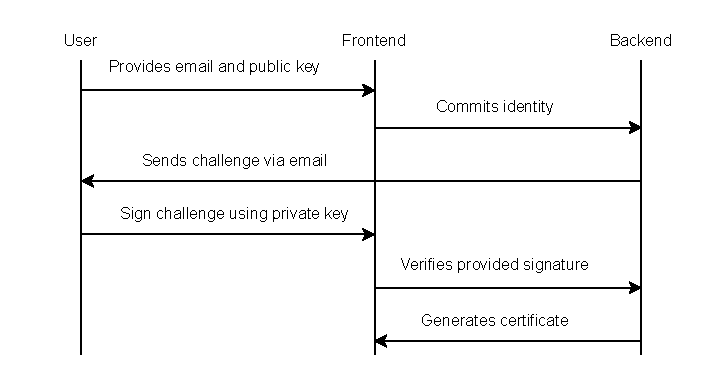
\includegraphics[keepaspectratio, width=\textwidth]{Pic/create_certificate.pdf}
    \caption{Identity commitment and certificate generation flow}
    \label{fig:certificate-creation-flow}
\end{figure}
When a user wants to revoke a certificate, the frontend sends a POST request to 
`/v1/certificate/revoke` containing the serial number of the certificate and the revocation 
signature. The backend validates the signature and confirms revocation through a JSON response.

\begin{figure}[h!]
    \centering
    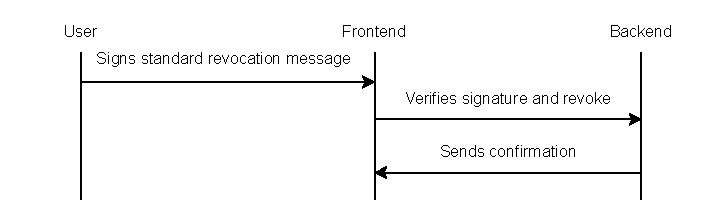
\includegraphics[keepaspectratio, width=\textwidth]{Pic/revoke_certificate.pdf}
    \caption{Certificate revocation flow}
    \label{fig:certificate-revocation-flow}
\end{figure}
Similarly, when a user wants to renew a certificate, the frontend sends a POST 
requests to `/v1/certificate/renew` containing renewal signatures and the serial number of the 
certificate. Successful renewal returns both confirmation and the renewed certificate.

\begin{figure}[h!]
    \centering
    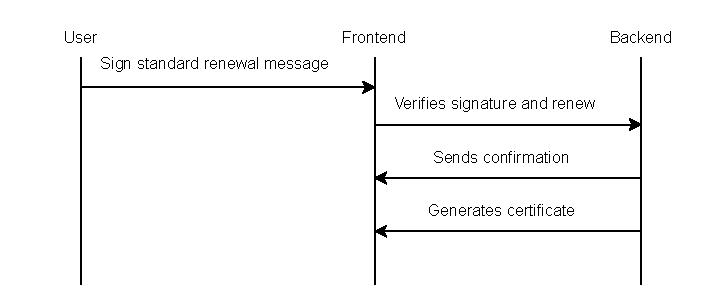
\includegraphics[keepaspectratio, width=\textwidth]{Pic/renew_certificate.pdf}
    \caption{Certificate renewal flow}
    \label{fig:certificate-renewal-flow}
\end{figure}

\subsection{HSM integration patterns}

The HSM integration follows secure communication patterns 
that ensure private key material never leaves the secure boundary:

\subsection{Key creation}
During system initialization, the CA creates a root key 
within the HSM using the AWS KMS CreateKey API. The key specification uses 
ECC NIST P-256 for its security and performance. The HSM generates the key 
pair entirely within secure hardware, returning only the key identifier.

\subsection{Certificate signing}
For each certificate signing operation, the CA 
constructs the certificate structure locally and sends it to the HSM via the 
KMS Sign API. The HSM performs the cryptographic signature using the stored 
private key and returns only the signature bytes. This pattern ensures the 
private key never exists outside the HSM boundary.

\subsection{Root certificate generation}
The system generates the CA's root certificate 
by creating the certificate structure and requesting HSM signing. The resulting 
self-signed root certificate establishes the trust anchor for all issued certificates.

\section{Signed responses}

To ensure response integrity and prevent tampering, the system implements 
OCSP-like signed responses for critical operations:

\subsection{Response structure}
Each signed response contains response data, 
signature algorithm identifier, Base64-encoded signature, and optional signing 
certificate chain. The response data includes nonces for replay protection 
and timestamps for freshness validation.

\subsection{Certificate status responses}
When clients query certificate status, 
the CA constructs a response containing the serial number, status (good/revoked/unknown), 
update timestamps, and revocation details if applicable. The complete response 
is signed using the HSM to ensure authenticity.

\subsection{Revocation list responses}
Certificate Revocation List queries return 
signed responses containing the list of revoked certificates with pagination 
support. Each response includes update timestamps and replay protection nonces.

\section{Code Structure and organization}

The project follows a monorepo structure with clear separation between different 
services and components, enabling independent development and deployment while 
maintaining code organization.

\subsection{Backend service (ca/)}
This directory contains the complete Go-based Certificate Authority 
server implementation. This module includes the REST API server, HSM integration, 
database operations, and email services. The structure follows Go's standard 
project layout with clear separation between commands, internal packages, and 
configuration. It is organized as follows:
\begin{itemize}
    \item \textbf{cmd/}: Contains the main application entry point and service 
    initialization logic.
    \item \textbf{internal/}: Core business logic modules including configuration, 
    database operations, HSM integration, email services, and HTTP server implementation.
    \item \textbf{handler/}: RESTful API endpoint implementations organized by 
    functionality (e.g., certificate operations, health monitoring).
\end{itemize}

\subsection{Frontend application (ui/)}
This directory contains the Next.js-based web interface 
providing user-facing certificate management capabilities. The structure follows 
Next.js App Router conventions with organized pages, components, and utility 
functions for cryptographic operations.
In particular:
\begin{itemize}
    \item \textbf{app/}: Contains the main application entry point, routing, and 
    layout definitions. The directory structure follows Next.js conventions with 
    pages organized by functionality.
    \item \textbf{components/}: Reusable UI components such as forms, buttons, 
    and modals used across different pages.
    \item \textbf{utils/}: Utility functions for cryptographic operations, API 
    communication, and data formatting.
\end{itemize}

\subsection{Certificates (dev-certs/)}
This directory, initially empty, contains the root certificate generated by the CA.

\subsection{Deployment configuration}
In the root directory of the project there are files including Docker Compose 
orchestration, MongoDB configuration, and environment setup scripts for 
containerized deployment.

\section{Dependencies and libraries}

The system uses external dependencies to provide robust functionality 
while minimizing security risks and maintaining code quality.

\subsection{Backend dependencies}
Go 1.21+ provides all the packages required for cryptographic operations, thanks to 
its standard library including crypto/x509, crypto/rsa, crypto/ecdsa, but also net/http 
for API server functionality.
To integrate MongoDB, we decided to use the official MongoDB Go driver (go.mongodb.org/mongo-driver/v2) 
as it provides secure and comprehensive access to MongoDB features, including 
document-oriented data storage, indexing, and querying capabilities.
For the HSM, we decided to opt for the official AWS SDK Go library (github.com/aws/aws-sdk-go-v2) 
as it provides programmatic access to AWS KMS for secure key management and signing 
operations.
Lastly, we opted for Resend Go package as it is the official client of the email delivery service
we decided to use.


\subsection{Frontend dependencies}

At the core we decided to use Next.js 15 with React 19 as it provides easy routing and
lots of UI packages with pre-built components, which allowed us to speed up the development process.
We opted for Web Crypto API (browser native) to handle 
client-side cryptographic operations without requiring external libraries.

\subsection{Infrastructure dependencies}

We opted for Docker and Docker Compose as they allow for easy and consistent deployment 
environments with isolated service containers. For the database, as we wanted a document-based one,
we decided to use MongoDB since we were already familiar with it and it provides document-oriented 
data storage with indexing, and querying capabilities for scalable management.
For the HSM, the only free solution we found was LocalStack KMS, which provides a local HSM emulation
for development and testing environments without requiring cloud resources, but emulating the AWS KMS API.

\subsection{Security and compliance dependencies}

All selected dependencies prioritize security and maintain active development 
with regular security updates. The minimal dependency approach reduces attack 
surface while leveraging proven, well-maintained libraries from reputable sources. 
Cryptographic operations rely primarily on standard library implementations 
and certified hardware modules rather than third-party cryptographic libraries, 
ensuring compliance with security standards and reducing implementation risks.